\documentclass[11pt,a4paper]{article}
\usepackage[T1]{fontenc}
\usepackage[utf8]{inputenc}
\usepackage{lmodern,microtype}
\usepackage{amsmath,amssymb,amsthm,mathtools,bm}
\usepackage{booktabs,array,tabularx,longtable}
\usepackage{graphicx,float,caption}
\usepackage{xcolor}
\usepackage[margin=20mm]{geometry}
\usepackage{enumitem,fancyhdr}
\usepackage[hidelinks,unicode=true]{hyperref}
\hypersetup{
 pdftitle={FIN ST203--ST217: Schedule Obstructions, Fluctuation Selection, and Diffusion Geometry},
 pdfauthor={Krzysztof Żuchowski},
 pdfsubject={Analytical, interval, and computational execution of FIN programs ST203--ST217},
 pdfkeywords={FIN, fractal information, semigroup schedule, Blackwell lattice, symmetry breaking, pseudo-arclength, quantum recovery, diffusion geometry, hidden Markov model, sample complexity}
}
\setlength{\parindent}{0pt}
\setlength{\parskip}{0.48em}
\setlength{\emergencystretch}{2em}
\setlength{\headheight}{14pt}
\setlist[itemize]{leftmargin=1.55em,itemsep=0.14em,topsep=0.2em}
\setlist[enumerate]{leftmargin=1.75em,itemsep=0.14em,topsep=0.2em}
\pagestyle{fancy}\fancyhf{}
\lhead{FIN ST203--ST217}\rhead{Release 10.71}\cfoot{\thepage}
\newtheorem{theorem}{Theorem}[section]
\newtheorem{proposition}[theorem]{Proposition}
\newtheorem{corollary}[theorem]{Corollary}
\newcommand{\proven}{\textcolor{green!40!black}{\textbf{[PROVEN]}}}
\newcommand{\strong}{\textcolor{blue!70!black}{\textbf{[STRONG EVIDENCE]}}}
\newcommand{\conditional}{\textcolor{violet!65!black}{\textbf{[CONDITIONAL]}}}
\newcommand{\openstatus}{\textcolor{red!72!black}{\textbf{[OPEN]}}}
\newcommand{\blocked}{\textcolor{orange!82!black}{\textbf{[BLOCKED]}}}
\newcommand{\boundarymark}{\textcolor{orange!82!black}{\textbf{[BOUNDARY]}}}
\newcommand{\resultbox}[1]{\begin{center}\fcolorbox{blue!60!black}{blue!4}{\parbox{0.92\textwidth}{#1}}\end{center}}

\begin{document}
\pagenumbering{gobble}
\begin{titlepage}
\centering
\vspace*{0.60cm}
{\LARGE\bfseries FIN ST203--ST217\par}
\vspace{0.24cm}
{\Large Schedule Obstructions, Fluctuation Selection, and Diffusion Geometry\par}
\vspace{0.34cm}
{\large Exact semigroup-history nonidentifiability, the complete Blackwell partition lattice, a strict-covariant fluctuation candidate, forty validated pseudo-arclength steps, negative-orientation recovery, a finite-time selector speed limit, a carrier-scale-invariant nonlinear response, a 2,744-box adaptive cover, correlated multimode sampling bounds, global joint-factor nonuniqueness, an asymptotic observed-HMM rate bracket, a time-dependent local-reset no-go, and dimensionless diffusion geometry\par}
\vspace{0.65cm}
{\Large Krzysztof \.{Z}uchowski\par}
\vspace{0.16cm}
{\large Independent Researcher --- Fractal Information Theory Project\par}
{\large ORCID: 0009-0002-0909-3613\par}
\vspace{0.45cm}
{\large FIN Release 10.71 --- Version 1.0.0\par}
{\large August 11, 2026\par}
\vfill
\begin{minipage}{0.93\textwidth}
\textbf{Research question.} If the strict operator supplies a continuous family of compression layers, can it also choose their discrete fractal history? Can a fluctuation generated from the strict operator solve the selector problem? Does the layer tower induce an intrinsic geometry even without meters or a Planck scale?\par
\textbf{Methods.} Semigroup identifiability, exact finite partition lattices, Ornstein--Uhlenbeck covariance equations, equivariant replicator dynamics, outward interval pseudo-arclength continuation, Pauli twirling, comparison principles for controlled Markov systems, jet invariants, adaptive Krawczyk covers, Fisher matrices with cluster correlation, exact matrix-factor counterexamples, almost-additive HMM bounds, commutator injectivity, and diffusion-map asymptotics.\par
\textbf{Epistemic rule.} A continuous layer family is not a selected layer history. Symmetric stochastic selection is not canonical orientation. Diffusion distance is not a dimensionful spacetime metric. Local structural validation is not external evidence.\par
\textbf{Repository snapshot.} Audited tracked base commit \texttt{4f388307bdaff902114c020e1adf54307280e7ec}. Local research artifacts are covered by a separate SHA-256 manifest.\par
\textbf{Repository.} \url{https://github.com/hyconiek/Fractal-Nadsoliton-Theory}\par
\textbf{License.} CC BY 4.0.
\end{minipage}
\end{titlepage}
\pagenumbering{arabic}

\begin{abstract}
Programs ST203--ST217 continue the strict-generated layer analysis. ST203 proves an exact obstruction: every hierarchy composed only of strict heat maps satisfies
\[
e^{-t_nA}\cdots e^{-t_1A}=e^{-(t_1+\cdots+t_n)A}.
\]
The final layer therefore identifies only total semigroup time. It cannot reveal the number, ordering, or ratios of increments. Even among four-layer geometric schedules, every ratio $r>0$ can be assigned a base increment giving the same final map. Thus the strict heat family is an internal layer mechanism, but no preferred dyadic or fractal history follows from its final composite.

ST204 enumerates the complete deterministic Blackwell lattice generated by the four minimal sufficient atoms of ST191. It is the fifteen-element partition lattice $\Pi_4$, with block-count distribution $1,7,6,1$ and 31 cover edges. ST205 constructs the strict-covariant fluctuation
\[
d\xi=-A\xi\,dt+\sqrt{2A}\,dB
\]
on the mean-zero sector. Its invariant covariance is $Q=I-J/12$. Coupling a sample to the ST192 feedback selects all twelve orbit members across 120 runs, but exact $C_{12}$ and inversion symmetry forces equal ensemble probabilities and forbids a canonical orientation. This supplies a mathematically natural fluctuation shape, not a QW-2191 discharge.

ST206 validates forty two-sided pseudo-arclength steps on one nonuniform branch. Every hyperplane corrector has an outward Krawczyk certificate; the minimum seven-row Jacobian rank margin is $7.15\times10^{-4}$. ST207 solves a negative-polar-orientation Pauli channel globally over all CPTP recoveries. Pauli twirling reduces the problem to a linear program and proves optimum entanglement fidelity $3/10$.

ST208 proves a finite-time selector speed limit under bounded field and relaxation rate. ST209 identifies the minimal carrier-scale-invariant nonlinear jet ratio
\[
I_{12}=\frac{R_{12}}{11!R_2^6}=\frac{g}{A_{jj}^6},
\]
and proves that no lower-order local jet can identify $g$. ST210 adaptively refines the failed ST197 grid and interval-certifies all $14^3=2744$ boxes of a nuisance cube of halfwidth $2\times10^{-4}$. ST211 derives simultaneous Fourier-mode Fisher bounds and a cluster-correlation design effect; the deepest displayed iid lower bound exceeds $1.39\times10^{10}$ samples.

ST212 gives an exact circle of global nearest-joint-factor minimizers, refuting unconditional global uniqueness. ST213 proves existence of the exact observed-HMM Hellinger rate using quasi-multiplicativity and gives the rigorous $n=12$ asymptotic bracket $[0.6765651,0.8498519]$. ST214 promotes ST201 to a time-dependent no-go: pointwise energy-conserving controls in the declared 60-dimensional local span vanish almost everywhere. ST215 proves that strict heat-kernel rows define a genuine dimensionless diffusion metric and that, after spectral rescaling, it converges to the chordal metric of the first Fourier circle. ST216 formally separates viewing, sufficiency, invertibility, and stable reconstruction. ST217 remains correctly blocked by the absence of external evidence.

The central conclusion is two-sided. FIN now has an intrinsic dimensionless layer geometry, but its present symmetric functional calculus supplies neither a preferred layer history nor a canonical branch orientation. No Planck scale, physical spacetime, dimensional clock, external result, legacy-role transfer, Standard Model, gravity, $L_{\rm total}$, or Theory-of-Everything closure follows.
\end{abstract}

\textbf{Status vocabulary.} \proven{} denotes exact analytic, finite, or outward-interval proof in scope. \conditional{} marks supplied additional dynamics or controls. \strong{} denotes numerical evidence. \blocked{} records unavailable external evidence. \boundarymark{} records a non-implication.

\tableofcontents
\newpage

\section{Core discipline and present question}

The strict working object remains
\begin{equation}
W_{xx}=0,\qquad
W_{xy}=\frac{\cos(0.18575d(x,y)+0.16250)}{1+d(x,y)^{9/5}}\quad(x\ne y),
\qquad A=sI-W,
\label{eq:strict}
\end{equation}
where $s=2\sum_{d=1}^5W(d)+W(6)\approx1.660307278766099$. Hence
\[
\langle f,Af\rangle=\frac12\sum_{x,y}W_{xy}|f_x-f_y|^2\ge0.
\]

The legacy ontological kernel remains an intermediate bridge object. No legacy physical formula is silently transferred to~\eqref{eq:strict}. The nadsoliton itself remains primordial fractal information in a solitonic state; there is no informational substrate beneath it.

Release 10.70 proved that $A$ generates a continuous family of soft layers $e^{-tA}$. The present batch asks whether the family can select its own history, whether its symmetry-compatible fluctuations can select a canonical state, and whether it induces a useful intrinsic geometry.

\resultbox{\textbf{Central result.} The strict operator supplies a layer semigroup and a diffusion geometry, but not a unique fractal schedule. All heat histories with the same total parameter cast the same final shadow. A strict-covariant fluctuation can initiate spontaneous branch selection, but its invariant symmetry makes every branch equiprobable and therefore cannot generate a canonical orientation.}

\section{Outcome matrix}
\small
\begin{longtable}{@{}p{0.06\textwidth}p{0.23\textwidth}p{0.33\textwidth}p{0.30\textwidth}@{}}
\toprule ID & Target & Result & Boundary\\\midrule\endfirsthead
\toprule ID & Target & Result & Boundary\\\midrule\endhead
ST203 & Layer schedule & \proven{} exact collapse to total semigroup time & Noncommuting/refinement data outside scope\\
ST204 & Operational quotients & \proven{} complete fifteen-element lattice & Preparation-family relative\\
ST205 & Endogenous fluctuation & \conditional{} strict covariance; \proven{} no canonical branch & Brownian law/coupling supplied\\
ST206 & Global continuation step & \proven{} 40 local pseudo-arclength boxes & One finite branch segment\\
ST207 & Negative-orientation recovery & \proven{} global CPTP optimum $3/10$ & Pauli-covariant class\\
ST208 & Finite-time selector & \proven{} exact speed bound in reduced class & Not minimum-dissipation control\\
ST209 & Nonlinear response & \proven{} scale-invariant ratio and jet minimality & Response access supplied\\
ST210 & Adaptive nuisance cover & \proven{} all 2744 boxes at halfwidth $2\times10^{-4}$ & Maximal domain open\\
ST211 & Multimode sampling & \proven{} local Fisher minimax and design effect & Declared count model\\
ST212 & Joint-factor uniqueness & \proven{} continuum counterexample & Zero odd-part gap\\
ST213 & HMM asymptotic rate & \proven{} existence and rigorous bracket & Conservative; $s=1/2$ only\\
ST214 & Controlled reset & \proven{} pointwise-conserving time-dependent no-go & Net-only conservation open\\
ST215 & Layer geometry & \proven{} metric and circle limit & Dimensionless, noncausal\\
ST216 & Observer language & \proven{} four distinct operational notions & Physical family unspecified\\
ST217 & External evidence & \blocked{} correct refusal & No laboratory record\\
\bottomrule
\end{longtable}
\normalsize

\section{ST203: why the final layer cannot reveal its history}

\begin{theorem}[Heat-schedule collapse]
For every finite nonnegative schedule $(t_1,\ldots,t_n)$,
\[
\prod_{j=n}^{1}e^{-t_jA}=e^{-TA},\qquad T=\sum_{j=1}^nt_j.
\]
Consequently the final composite depends on $T$ only. It contains no information about the number, ordering, or ratios of increments.
\end{theorem}

The theorem is an immediate consequence of using one generator. Numerically, the single schedule $[3.75]$, four uniform increments, the dyadic schedule $[0.25,0.5,1,2]$, and the irregular schedule $[0.1,0.2,0.45,3]$ agree to within $5.6\times10^{-16}$.

For four geometric layers $t_j=t_0r^{j-1}$, every $r>0$ admits
\[
t_0=\frac{T}{1+r+r^2+r^3}.
\]
Thus $r=1/4,1/2,1,2,4$ all produce the same final map after choosing their respective bases.

\begin{figure}[H]\centering
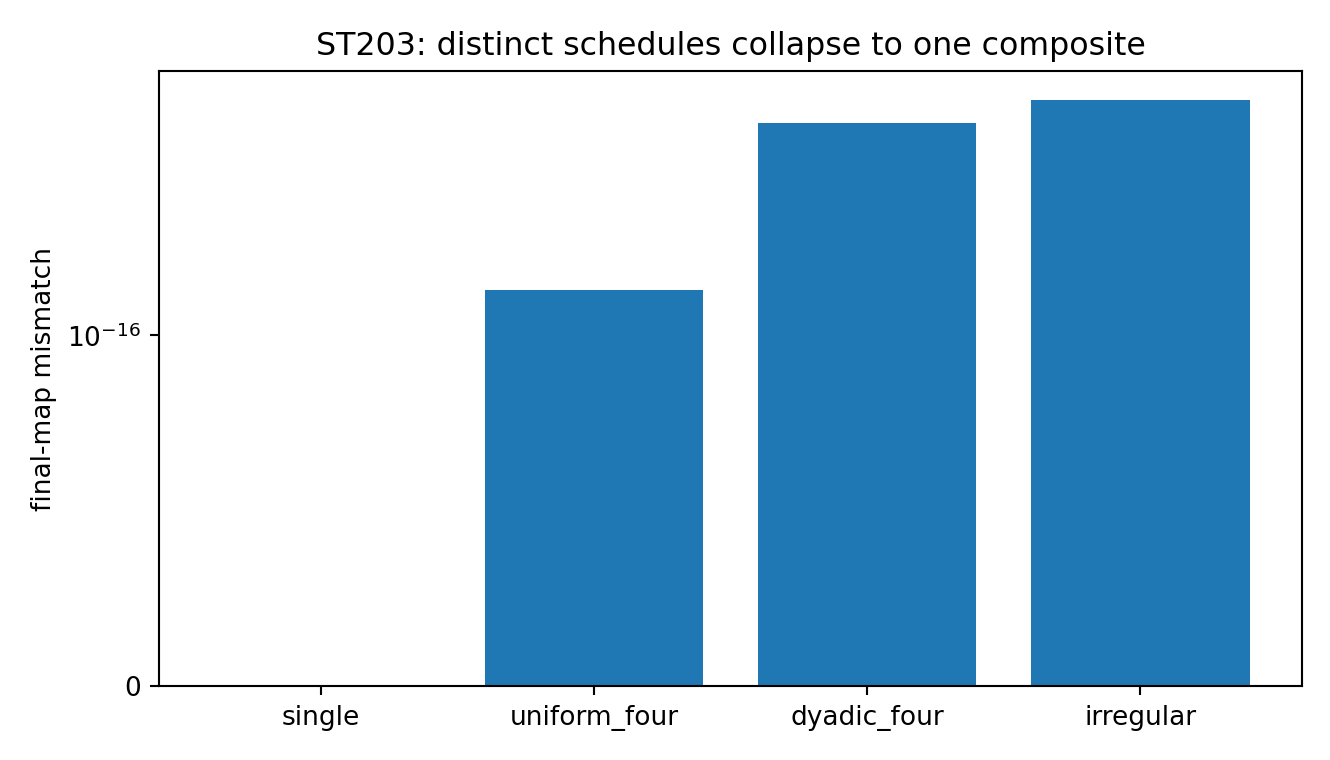
\includegraphics[width=.72\textwidth]{FIN_ST203_ST217_Figures/st203_schedule_collapse.png}
\caption{ST203. Distinct layer histories are operationally identical at the same final semigroup parameter.}
\end{figure}

Intermediate observations can recover the increments through spectral log-ratios if $A$ and its normalization are fixed. They do not select those increments. A preferred fractal history requires at least one of: a noncommuting generator, a refinement label retained between stages, a state-dependent layer law, or a new scale-selection axiom.

\section{ST204: the complete Blackwell experiment lattice}

ST191 found four minimal likelihood-proportionality atoms. Every deterministic coarse experiment is therefore a set partition of these four atoms.

\begin{theorem}[Blackwell partition lattice]
The deterministic coarse experiments form $\Pi_4$. Experiment $P$ Blackwell-dominates $Q$ exactly when partition $P$ refines partition $Q$. Meet is common refinement; join is the transitive closure of the two equivalence relations.
\end{theorem}

The exact enumeration gives
\[
|\Pi_4|=15,
\]
with block-count distribution
\[
1\ (1\text{ block}),\quad7\ (2),\quad6\ (3),\quad1\ (4),
\]
and 31 Hasse cover edges. Only the four-block element is sufficient for the original full three-hypothesis experiment. The remaining fourteen are genuine information-loss patterns, ordered by post-processing.

This gives an exact atlas of possible observational quotients for one FIN-like experiment. It is not universal: changing the preparation or instrument family changes the likelihood columns and may change the atoms themselves.

\section{ST205: an operator-shaped fluctuation still cannot orient the world}

On the mean-zero sector, define
\[
d\xi=-A\xi\,dt+\sqrt{2A}\,dB_t,
\qquad Q=I-\frac{J}{12}.
\]

\begin{theorem}[Strict-covariant fluctuation]
The covariance $Q$ solves
\[
AQ+QA=2A.
\]
Hence the process has a centered invariant Gaussian law with covariance $Q$. Because $A$ is circulant and inversion-even, this law is invariant under $C_{12}$ and inversion.
\end{theorem}

The computed Lyapunov residual is $3.21\times10^{-14}$. Sampling the invariant law and applying the ST192 positive feedback selects every one of the twelve vertices in 120 runs. The smallest final maximum probability equals one at stored precision.

\begin{figure}[H]\centering
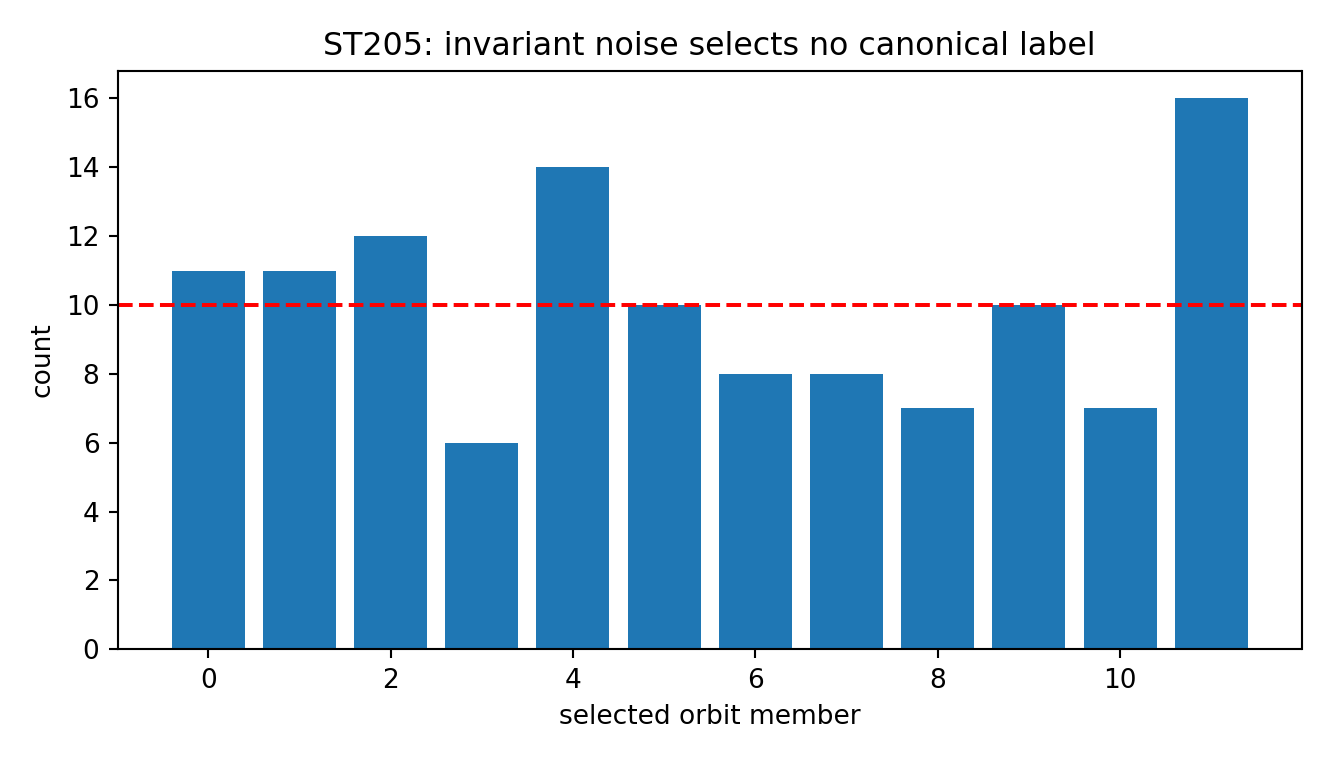
\includegraphics[width=.73\textwidth]{FIN_ST203_ST217_Figures/st205_branch_counts.png}
\caption{ST205. A finite sample fluctuates across orbit members, while the invariant ensemble contains no preferred label.}
\end{figure}

\begin{corollary}[Symmetric-noise selector obstruction]
If both the fluctuation law and the selection dynamics are equivariant and the twelve branches form one transitive orbit, all exact branch probabilities are equal. No canonical direction or origin can emerge at the ensemble-law level.
\end{corollary}

The result advances the selector analysis: $A$ naturally supplies a covariance shape. It does not supply the Brownian premise, noise strength, or coupling to feedback. More importantly, symmetry-compatible noise solves random realization, not canonical orientation. QW-2191 remains open.

\section{ST206: validated pseudo-arclength continuation}

The stationary equation has seven equations in eight variables $(q_0,\ldots,q_6,\kappa)$. ST206 begins at a certified mode-one state adjacent to the uniform amplitude $0.2914980865$ and traces both tangent directions with arc step $0.002$.

Each corrector solves the stationary system plus the pseudo-arclength hyperplane
\[
t_n^T(x-x_{\rm pred})=0.
\]

\begin{theorem}[Validated two-sided segment]
All forty correctors pass outward Krawczyk inclusion. The smallest nonzero singular value of the seven-row stationary Jacobian is
\[
7.1526866\times10^{-4},
\]
and the minimum consecutive tangent alignment is $0.9999749675$. No rank collision occurs on the traced segment.
\end{theorem}

\begin{figure}[H]\centering
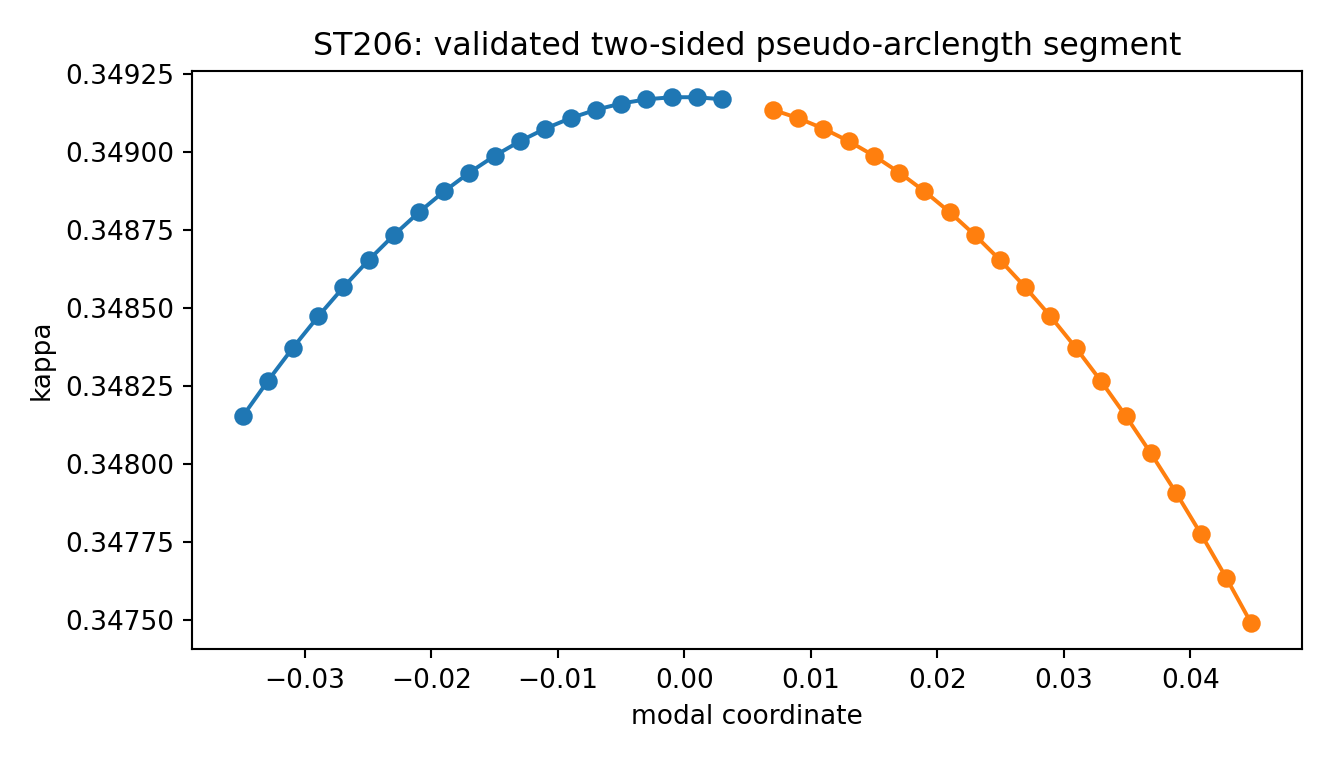
\includegraphics[width=.72\textwidth]{FIN_ST203_ST217_Figures/st206_pseudo_arclength.png}
\caption{ST206. The interval-certified branch segment in modal-coordinate--$\kappa$ projection.}
\end{figure}

This is stronger than fixed modal slices because the parameterization can pass ordinary projection folds. It remains one local segment in the reflection-even sector. It is not a global branch graph, collision census, orbital-stability theorem, or physical particle result.

\section{ST207: negative-orientation noncommuting recovery}

Consider the Pauli channel with exact probabilities
\[
(p_I,p_X,p_Y,p_Z)=\left(\frac1{10},\frac3{10},\frac3{10},\frac3{10}\right).
\]
Its Bloch matrix is $\operatorname{diag}(-1/5,-1/5,-1/5)$ and has determinant $-1/125$.

\begin{theorem}[Pauli-twirled global recovery]
Pauli-twirling any CPTP recovery preserves its entanglement fidelity against a Pauli channel and yields a Pauli recovery channel. The remaining objective is linear in four recovery probabilities. Therefore a globally optimal recovery is a Pauli unitary correcting a most likely error.
\end{theorem}

The optimum over all CPTP recoveries, including nonunital maps, is
\[
\boxed{F_e^*=\frac3{10}},
\]
attained by $X$, $Y$, or $Z$ correction. These errors are mutually noncommuting as operators. This closes one negative-orientation family but not arbitrary non-Pauli or generic nonunital channels.

\section{ST208 and ST209: finite-time selection and the minimal nonlinear datum}

\subsection{A selector speed limit}

In the symmetric twelve-state reduction, let $x$ be the preferred-vertex probability and
\[
\dot x=r(t)[\pi(t)-x],\qquad0\le r(t)\le R,qquad \pi(t)\le\pi_B.
\]

\begin{theorem}[Fastest bounded selector]
For $x_f<\pi_B$,
\[
T\ge\frac1R\log\frac{\pi_B-x_0}{\pi_B-x_f}.
\]
Constant maximal control $r=R$, $\pi=\pi_B$ attains equality. Targets $x_f\ge\pi_B$ are unreachable.
\end{theorem}

For $\beta h\le4$, $R=1$, and $x_0=1/12$, one has $\pi_B=0.8323123443$. The minimum times to reach $x_f=0.2,0.4,0.6,0.8$ are approximately $0.1693,0.5496,1.1706,3.1433$. Under the saturating constant control, integrated entropy production is
\[
D(x_0\|\pi_B)-D(x_f\|\pi_B).
\]
This is a fastest-control theorem, not the general minimum-dissipation solution at fixed time.

\subsection{Carrier-scale-invariant response}

Let $R_2=A_{jj}$ and $R_{12}=11!g$ be the local quadratic and twelfth responses. Under the coordinate rescaling $\psi'=c\psi$,
\[
R_2\mapsto c^{-2}R_2,qquad R_{12}\mapsto c^{-12}R_{12}.
\]

\begin{theorem}[Minimal invariant jet]
The ratio
\[
I_{12}=\frac{R_{12}}{11!R_2^6}=\frac{g}{A_{jj}^6}
\]
is invariant under scalar carrier-coordinate reparameterization. Since the potentials $V_g$ have identical jets through order eleven, a nonzero twelfth-order response is the lowest local jet datum capable of identifying the ratio.
\end{theorem}

The code verifies invariance for $g=0.1,1,10$ and scales $c=1/4,1/2,2,4$. This identifies a dimensionless coupling ratio if the response is available; it does not derive $g$ from $A$.

\section{ST210 and ST211: adaptive continuation and correlated multimode sampling}

\subsection{The nuisance cube reaches halfwidth \texorpdfstring{$2\times10^{-4}$}{2e-4}}

The failed $7^3$ grid at the ST197 boundary is refined once in every coordinate, equivalently producing $14^3=2744$ child boxes with local halfwidth $1.42857\times10^{-5}$.

\begin{theorem}[Adaptive complete cover]
Every child passes interval Krawczyk inclusion. Therefore the declared stationary root exists uniquely throughout the full nuisance cube of global halfwidth
\[
2\times10^{-4}.
\]
The smallest inclusion margin is $9.4713930\times10^{-4}$.
\end{theorem}

\begin{figure}[H]\centering
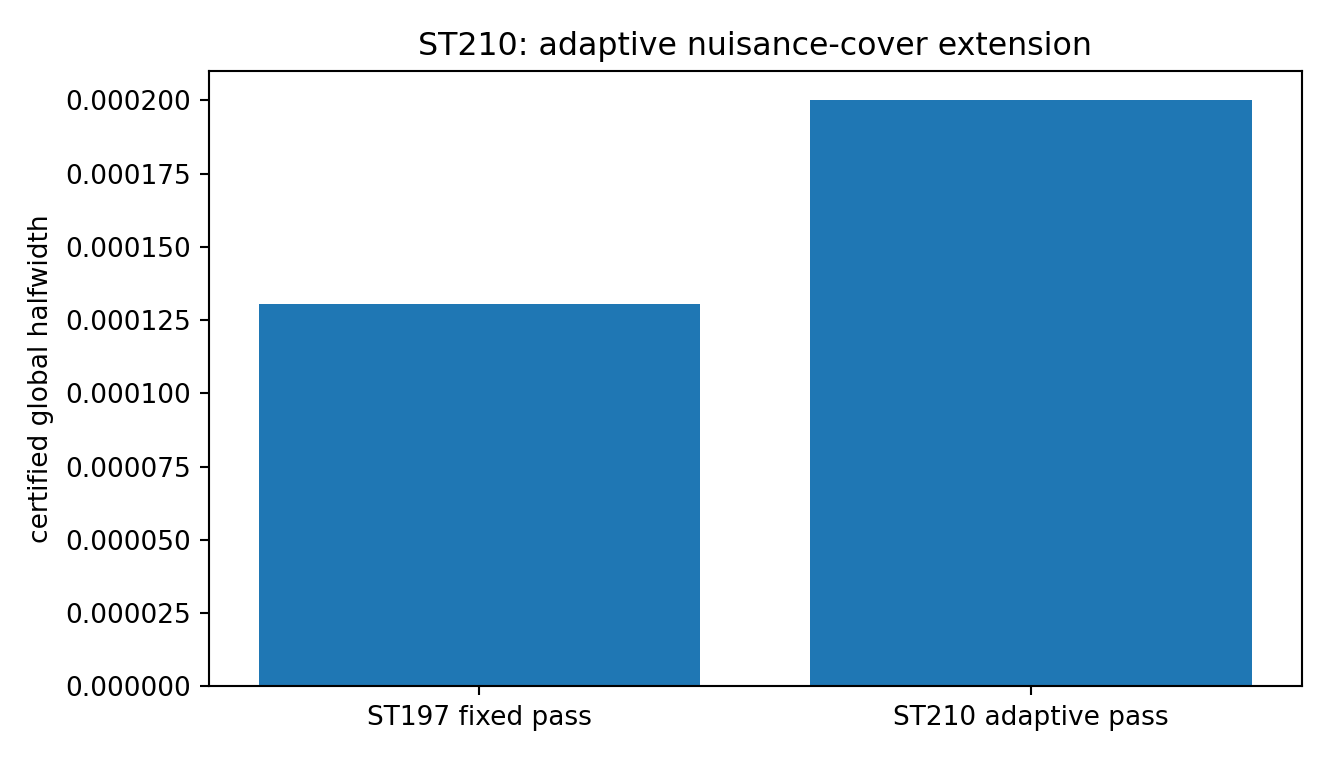
\includegraphics[width=.66\textwidth]{FIN_ST203_ST217_Figures/st210_adaptive_cover.png}
\caption{ST210. Adaptive subdivision extends the certified halfwidth beyond the fixed-grid failure.}
\end{figure}

This confirms that the ST197 upper failure was a method boundary, not root loss.

\subsection{Six modes under correlated counts}

At the uniform multinomial state, let six orthonormal Fourier contrasts be transmitted with attenuations $\sigma_k$. Their per-sample Fisher matrix is
\[
J_1=\operatorname{diag}(12\sigma_k^2).
\]

\begin{theorem}[Worst-mode sampling bound]
For $N$ iid samples, the largest directional Cram\'er--Rao variance is at least
\[
\frac1{12N\min_k\sigma_k^2}.
\]
For exchangeable clusters of size $m$ with intracluster correlation $\rho$, the necessary count is multiplied by
\[
1+(m-1)\rho.
\]
\end{theorem}

At twelve soft layers the deepest attenuation is $2^{-12}$. Standard deviation $0.01$ requires at least $13{,}981{,}013{,}334$ iid observations locally. With $m=20$ and $\rho=0.05$, the design effect is $1.95$ and the bound becomes $27{,}262{,}976{,}000$.

\begin{figure}[H]\centering
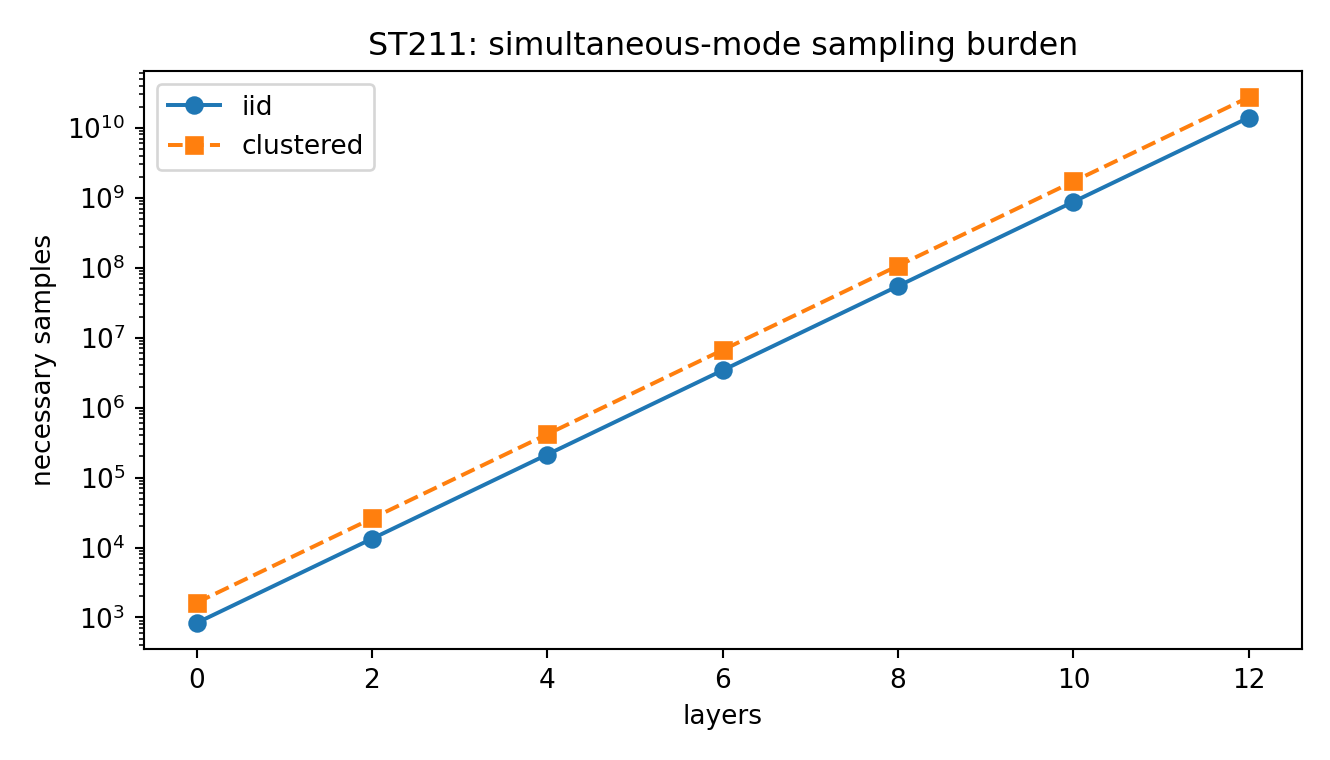
\includegraphics[width=.72\textwidth]{FIN_ST203_ST217_Figures/st211_multimode_samples.png}
\caption{ST211. Correlated observations further increase the already exponential deep-mode burden.}
\end{figure}

\section{ST212: global nearest-factor uniqueness is false without transversality}

For qubit involutions $X=n\cdot\sigma$, $Z=m\cdot\sigma$, anticommutation is $n\cdot m=0$. Take invertible raw targets
\[
X_0=Z_0=c\sigma_x,qquad c>0.
\]
The joint squared Frobenius objective is minimized by maximizing $e_x\cdot(n+m)$.

\begin{theorem}[Circle of global minimizers]
The inequality $e_x\cdot(n+m)\le\sqrt2$ is saturated for every unit vector $u\perp e_x$ by
\[
n=\frac{e_x+u}{\sqrt2},\qquad m=\frac{e_x-u}{\sqrt2}.
\]
Hence the globally nearest anticommuting pair is not unique; its minimizer set contains a circle.
\end{theorem}

For $c=0.8$, the exact minimum is $2.0345166004$, reproduced at twelve sampled circle points within $4.5\times10^{-16}$. The example has a zero odd-part gap, so it does not refute a future local uniqueness theorem using the full ST199 gap and transversality hypotheses.

\section{ST213: the exact observed-HMM rate exists}

Let $Z_n$ be the observed Hellinger coefficient. For the declared HMM, after any observed past one hidden transition places the next-state distribution $\nu$ within
\[
\frac3{10}\pi_j\le\nu_j\le\frac{12}{5}\pi_j
\]
componentwise relative to the stationary distribution $\pi$.

\begin{theorem}[Quasi-multiplicative observed coefficient]
For every $m,n\ge1$,
\[
\frac3{10}Z_mZ_n\le Z_{m+n}\le\frac{12}{5}Z_mZ_n.
\]
Consequently the limit
\[
R=\lim_{n\to\infty}-\frac1n\log Z_n
\]
exists, and every certified block value gives
\[
\frac{-\log Z_n-\log(12/5)}n\le R\le
\frac{-\log Z_n-\log(3/10)}n.
\]
\end{theorem}

Combining this with the exact-rational ST200 block enclosure at $n=12$ yields
\[
\boxed{0.67656507797\le R\le0.84985187311}.
\]

\begin{figure}[H]\centering
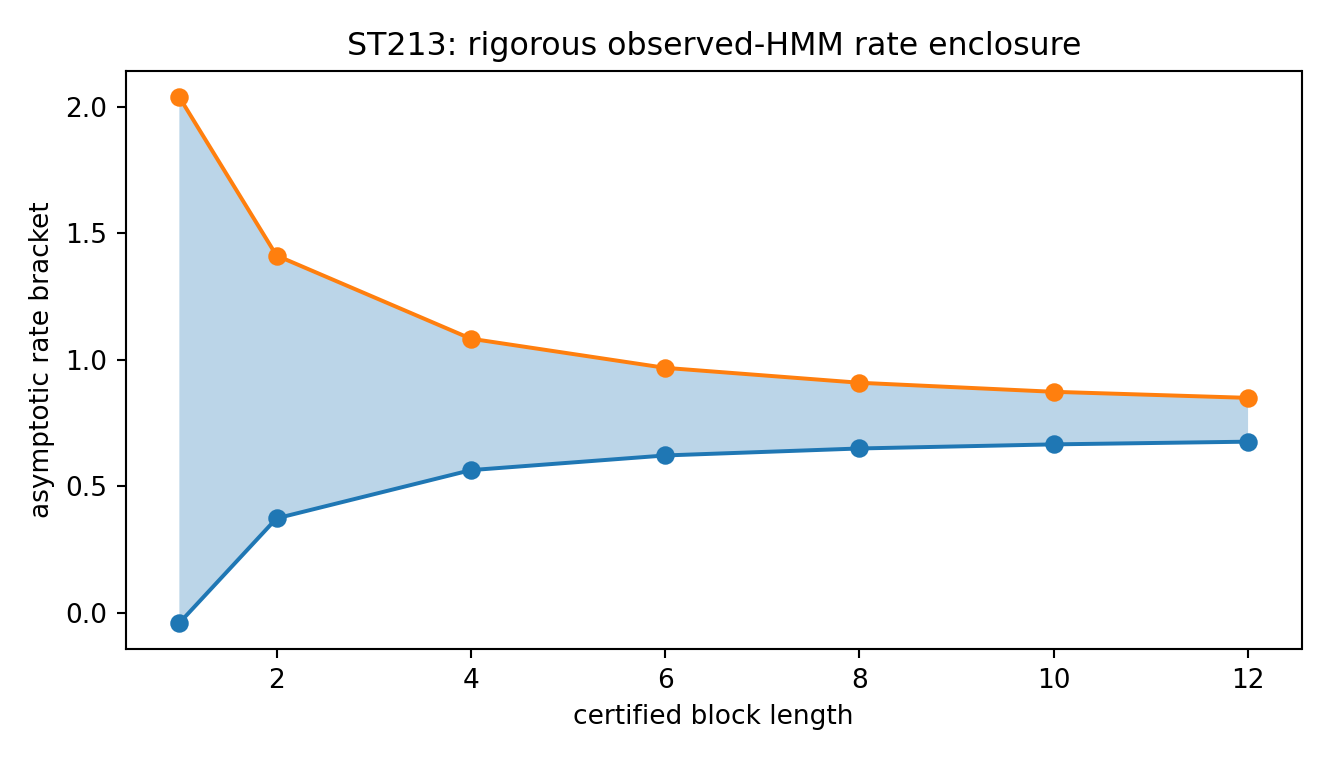
\includegraphics[width=.72\textwidth]{FIN_ST203_ST217_Figures/st213_hmm_rate_bracket.png}
\caption{ST213. Rigorous asymptotic observed-HMM rate brackets from finite exact blocks.}
\end{figure}

This proves existence and a quantitative interval, but it is conservative and fixes the Hellinger point $s=1/2$. It is not yet the optimized Chernoff exponent.

\section{ST214: time dependence does not help under pointwise conservation}

Let
\[
H_c(t)=\sum_{j=1}^{60}u_j(t)G_j
\]
belong at almost every time to the corresponding-pair Pauli span of ST201.

\begin{theorem}[Pointwise-conserving control no-go]
If
\[
[H_{\rm tot},H_c(t)]=0
\]
for almost every $t$, then $u(t)=0$ almost everywhere. Therefore the time-ordered exponential is the identity and no nontrivial reset occurs.
\end{theorem}

The proof uses the ST201 certified commutator-map lower singular bound $>6.324555$. Thus time-dependent coefficients do not evade an injective instantaneous conservation constraint. Net energy conservation only at the final time can allow cancellation among nonconserving segments and remains open.

\section{ST215: a dimensionless geometry emerges from the layer tower}

Define the heat-row embedding
\[
\Phi_t(i)=e_i^Te^{-tA}
\]
and diffusion distance
\[
D_t(i,j)=\|\Phi_t(i)-\Phi_t(j)\|_2.
\]

\begin{theorem}[Strict diffusion metric]
For every finite $t\ge0$, $e^{-tA}$ is invertible, so its rows are distinct. Hence $D_t$ is a genuine Euclidean metric. Circulant symmetry makes it depend only on cycle separation.
\end{theorem}

\begin{theorem}[First-mode circle limit]
Let $\lambda_1$ be the first positive strict Fourier eigenvalue. The spectral gap implies
\[
e^{t\lambda_1}D_t(0,d)\longrightarrow
\sqrt{\frac23}\left|\sin\frac{\pi d}{12}\right|.
\]
Thus the deep heat-layer geometry, after removing its global decay, converges to the chordal geometry of a circle represented by the first Fourier pair.
\end{theorem}

At $t=10$, the maximum discrepancy from the limit over separations $1,\ldots,6$ is $4.36\times10^{-8}$.

\begin{figure}[H]\centering
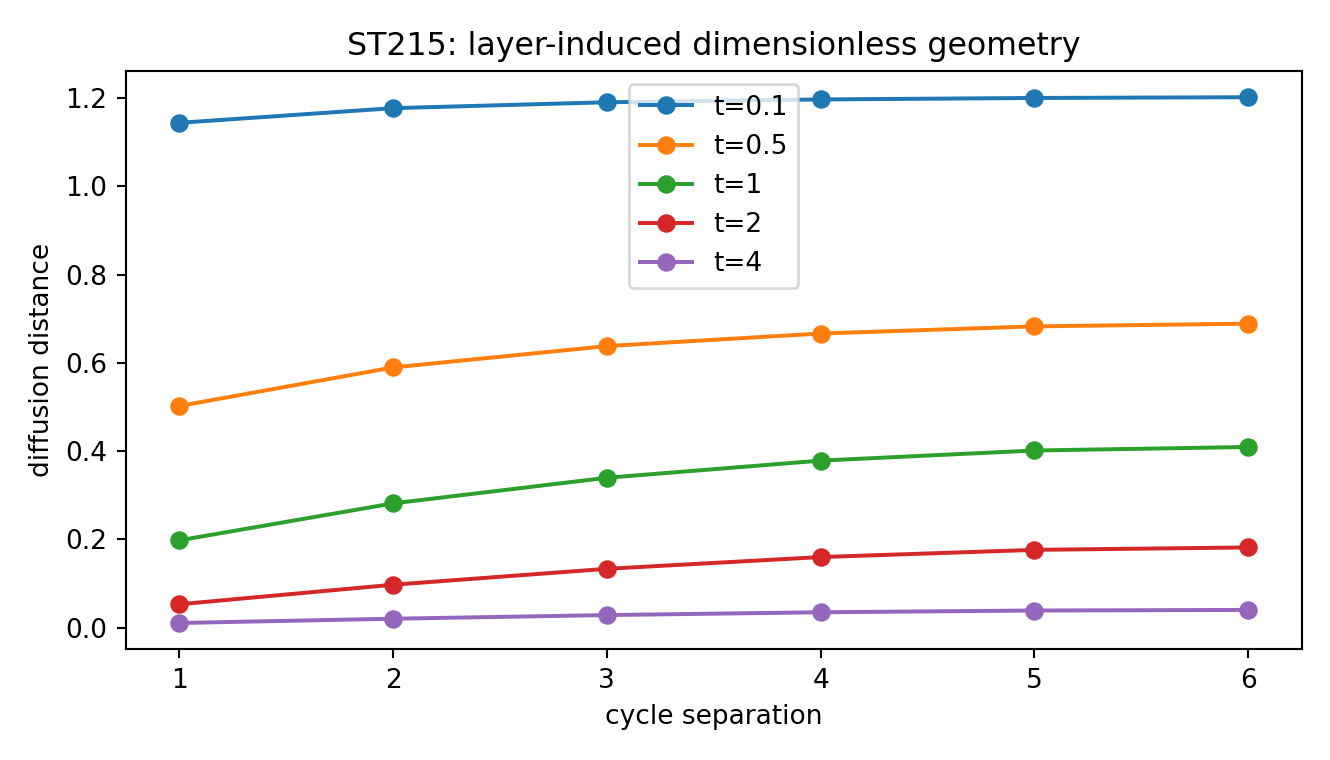
\includegraphics[width=.72\textwidth]{FIN_ST203_ST217_Figures/st215_diffusion_geometry.png}
\caption{ST215. The finite strict diffusion metrics contract while retaining the cyclic ordering of separations.}
\end{figure}

This is the strongest mathematical support in this batch for the intuition that later layers see lower scales through an induced effective geometry. The geometry remains dimensionless and Riemannian/Euclidean in construction. It supplies no meters, Lorentzian signature, causal cones, Planck length, or experimental spacetime identification.

\section{ST216 and ST217: observer language and the evidence stop}

\subsection{Four notions that must remain separate}

\begin{theorem}[Viewing versus reconstruction]
For a finite channel $C$:
\begin{enumerate}
\item an effect is \emph{viewable} exactly when it lies in $\operatorname{range}(C^T)$;
\item a decision experiment is \emph{sufficiently represented} when it admits the required Blackwell decoder;
\item a state model $M$ is \emph{exactly reconstructible} when $C|_M$ is injective;
\item reconstruction is \emph{stable} only when the restricted minimum singular value is positive, with noise amplification at least its reciprocal.
\end{enumerate}
These properties are logically distinct.
\end{theorem}

The hard $12\to3$ channel has rank three and a nine-dimensional kernel. It permits viewing selected coarse effects but not global reconstruction. The finite strict heat map is algebraically invertible, yet at the eight-layer parameter its exact spectral condition number is about $7.02\times10^{64}$. Thus invertibility does not imply operational reconstructibility.

\subsection{External evidence}

The immutable-record self-test remains structurally valid. No genuine laboratory record, independently frozen registration, calibration certificate, verified separation of provider/registrar/analyst, independent custody, or laboratory attestation exists. ST217 is therefore \blocked{}. Repeating local code cannot alter an external-evidence predicate.

\section{Interpretation: developed layers and deeper scales}

The user's intuition now decomposes into an increasingly precise chain:
\[
\begin{aligned}
\text{primordial informational nadsoliton}
&\xrightarrow{\text{spectral dynamics}}\text{soft layer family}\\
&\xrightarrow{\text{observation quotient}}\text{effective geometry and statistics}.
\end{aligned}
\]

The chain contains two proven internal arrows:
\begin{itemize}
\item $A$ generates heat-layer dynamics and mode attenuation;
\item heat-layer embeddings generate dimensionless diffusion metrics.
\end{itemize}

It also contains three unresolved source arrows:
\begin{itemize}
\item no strict law chooses a discrete hierarchy from the continuous family;
\item no symmetric strict fluctuation chooses a canonical orientation;
\item no dimension/operational theorem identifies one layer with observed physical spacetime.
\end{itemize}

The phrase ``we see lower scales through fractal layers'' is therefore mathematically defensible if it means that accessible statistics and geometry are images of deeper states under repeated spectral channels. It is not established if it means that the universe has a uniquely derived Planck-indexed tower or that current experimental physics has been reconstructed from it.

\subsection{New falsifications and boundaries}

\begin{itemize}
\item Final heat-map data cannot distinguish schedules with equal total parameter.
\item Strict-covariant centered fluctuations cannot create a canonical orbit label.
\item Global nearest-joint-factor uniqueness fails without a transversality gap.
\item Pointwise energy-conserving time-dependent controls do not evade an injective static commutator map.
\item Algebraic invertibility of a deep-layer channel does not imply stable empirical reconstruction.
\item Diffusion geometry does not generate dimensional or causal geometry by itself.
\end{itemize}

\section{Recommended programs ST218--ST232}

\begin{longtable}{@{}p{0.08\textwidth}p{0.12\textwidth}p{0.72\textwidth}@{}}
\toprule Program & Priority & Executable target\\\midrule\endfirsthead
\toprule Program & Priority & Executable target\\\midrule\endhead
ST218 & 1 & Test one noncommuting strict-derived layer generator; otherwise formalize the full $f(A)$ schedule no-go.\\
ST219 & 2 & Derive preparation-dependent Blackwell lattices for vertex, spectral, and nonlinear-response instruments.\\
ST220 & 3 & Classify all $\operatorname{Aut}(\mathbb Z_{12})$-covariant Gaussian and L\'evy fluctuations and prove their selector limit.\\
ST221 & 4 & Continue every certified nonuniform fold by pseudo-arclength and isolate all finite-segment singularities.\\
ST222 & 5 & Solve generic negative-orientation non-Pauli qubit recovery with replayable primal--dual certificates.\\
ST223 & 6 & Solve minimum-dissipation selector control at fixed finite time by interval dynamic programming.\\
ST224 & 7 & Construct a carrier-transport theorem for the normalized twelfth-response invariant.\\
ST225 & 8 & Extend adaptive nuisance coverage until certified root loss or a resource-bounded stop.\\
ST226 & 9 & Derive nonlocal and biased-estimator minimax bounds for simultaneous compressed modes.\\
ST227 & 10 & Prove a local nearest-joint-factor theorem under explicit gap and transversality premises.\\
ST228 & 11 & Sharpen the observed-HMM bracket by interval belief-space discretization.\\
ST229 & 12 & Test net-energy-conserving bang--bang reset sequences outside pointwise conservation.\\
ST230 & 13 & Compare strict diffusion geometry with resistance, Fisher, and spectral-projector metrics.\\
ST231 & 14 & Seek a refinement law preserving diffusion geometry up to scale without importing a length unit.\\
ST232 & 15 & Execute external validation only after a genuinely independent laboratory record exists.\\
\bottomrule
\end{longtable}

ST218 has the greatest foundational leverage: the schedule obstruction is complete for a single functional-calculus generator, so progress requires one genuinely new noncommuting or state-dependent typed object. ST220 is the sharp selector theorem. ST221, ST223, ST225, and ST228 are the strongest bounded computational continuations.

\section{Reproducibility and final claim ledger}

The release contains the research program, 26 live/serialized tests, the complete JSON result ledger, fifteen specialized packets, seven generated figures, summary CSV, source report, compiled PDF, release description, and SHA-256 manifest. Seed \texttt{20260812} controls only the finite ST205 fluctuation audit. Exact algebraic and interval statements do not depend on it.

\begin{itemize}
\item \proven{} a final heat layer identifies total semigroup time, not its schedule;
\item \conditional{} a strict-shaped Gaussian fluctuation can initiate spontaneous branch selection;
\item \proven{} its exact symmetry prevents canonical branch probabilities;
\item \proven{} strict heat rows define a dimensionless diffusion metric with a circle limit;
\item \openstatus{} no discrete scale law, physical unit, causal metric, or physical layer identification is derived;
\item \blocked{} no external laboratory evidence is present.
\end{itemize}

\resultbox{\textbf{Final answer.} The current FIN core can generate spectral layers and a dimensionless effective geometry, but its symmetric functional calculus erases the history of those layers and its symmetric fluctuations cannot canonically orient the selected branch. The next genuine theoretical advance must introduce or derive one typed object outside the present $f(A)$ and invariant-noise classes: a noncommuting refinement generator, a state-dependent scale law, or a non-premise symmetry-breaking source.}

\end{document}
